In the results presented so far we have used a rigid definition of failure (core dumps and hangs). This is necessary in order to meaningfully quantify our results, but it does leave out a section of softer errors that we encountered during our testing. Not presented in our results is the fact that a large number of applications behaved in ways that seemed very odd and outside of what the developers most likely intended. We include a few examples primarily because they show the types of errors that developers could find when debugging their code using our method. Furthermore, they offer some interesting behaviors that seem worth mentioning even though they are not part of our proper results. Figures 2-5 display some odd outputs for various calls.

\begin{figure}
	\caption{ld\_preload fig}
	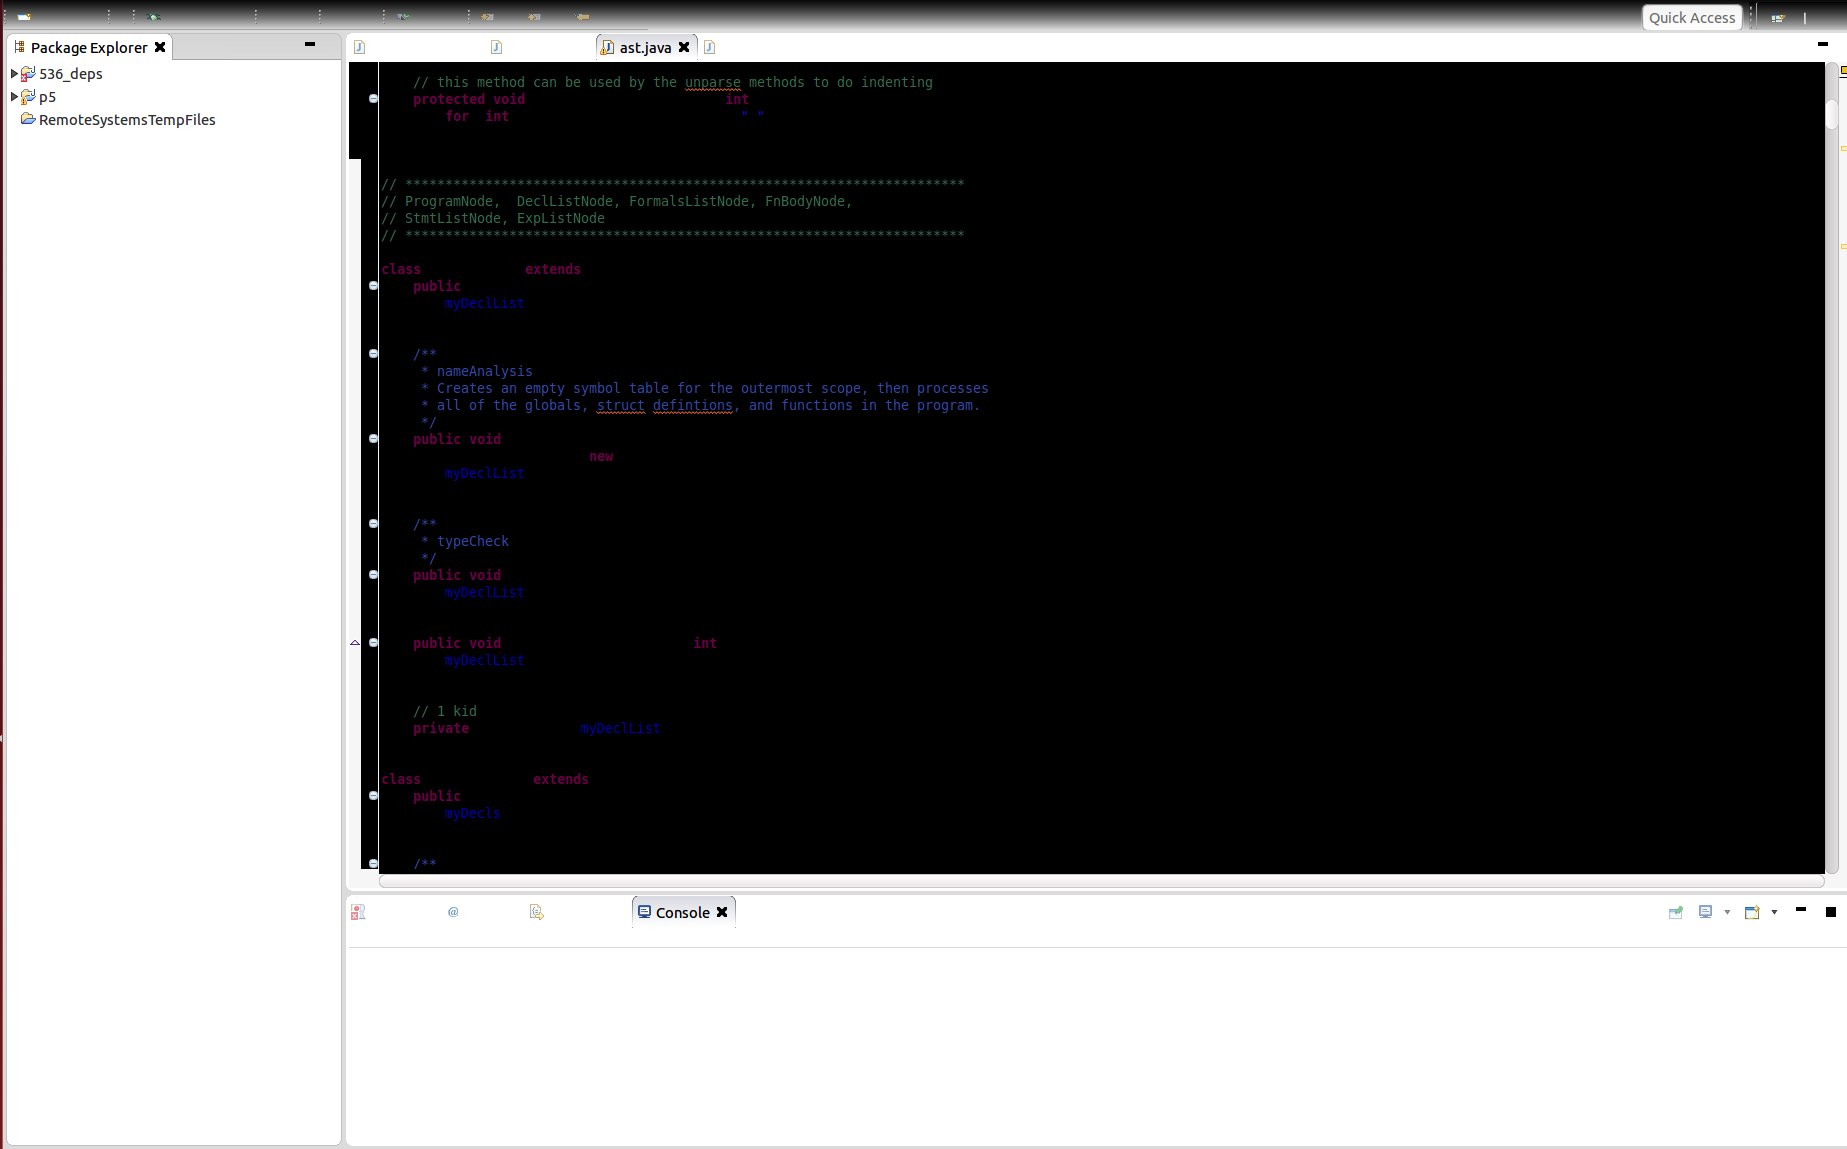
\includegraphics[width=\textwidth]{weird_eclipse.jpg}
\end{figure}